\documentclass[10pt,a5paper,final,]{memoir}%landscape,final,oneside,openany,twocolumn]{memoir}

\usepackage{abll}

\usepackage[left=3cm, right=3cm, top=2.7cm, bottom=2.7cm]{geometry}

\setlength{\parindent}{0pt}
\pagestyle{cleared}

\setcounter{secnumdepth}{0}
\def\thechapter{}
\setcolsepandrule{7.2cm}{0pt}


\newcommand{\songtitle}[1]{\section{\huge{#1}}\vspace*{3mm}}

\usepackage{pstricks}
\newrgbcolor{abllcolor}{.3 .4 .8}
\newcommand{\abll}[1]{{\textbf{\abllcolor{[abll: #1]}}}}


\begin{document}

%\vspace*{2.2cm}
\begin{center}
\begin{HUGE}
\textbf{Kantinens \\[3mm] julefrokost}
\end{HUGE}
\\[.6cm]
\begin{Large}
20. december 2013
\end{Large}
\end{center}
\vspace*{.01cm}
\begin{flushleft}
\begin{huge}
    Menu\footnote{Grundet studiefremdriftsreformen skal alle spise på normeret
    tid.}
\end{huge}
\\[.1cm]
%\hspace*{.4mm}\mbox{
%\texttt{\textbf{guest@diku\%} cat /proc/edible/menu | \hspace*{2.1cm} sed 's/salat/bacon/ig' }
%\begin{verbatim}
\newcommand{\course}[1]{\vspace*{4mm} \textbf{#1} \vspace{1mm}}
{\small
\course{Forret}
\\ Sild i enhver afskygning

\vspace{-.2cm}
\course{Hovedret} (buffet)
\\ Varm leverpostej
\\ Flæskeregoulade
\\ Frækkedeller
\\ Sprængt and
\\ Oksekødswraps
\\ Langtidsstegt lammekølle
\\ Kyllingesalat m. fetadressing
\\[2mm] Skaldyrssalat
\\ Lakseruller
\\[2mm] Vegetartærter
\\ Rødbede-tzatziki
\\ Brune kartofler
\\ Ovnbagte rodfrugter
\\ Rødkål-Appelsin salat
\\ Stuvet grønlangkål
\\ Waldorfsalat
\\ Kartoffelsalat
\\ Æble-julesalat-tranebær-salat med peberrodsdressing

\vspace{-.2cm}
\course{Dessert}
\\ Risalamande
}
%\end{verbatim}
\end{flushleft}


\newpage
\songtitle{I morgen er verden vor}
Se solen, der skinner på kalv og på kid\\
Se parken, der dufter af vår\\
Nu sammen vi hilser den nye tid\\
I morgen er verden vor!\\

Professoren giver af alt hvad han ved\\
Studerende sandheden får\\
Og æren den venter på os et sted\\
I morgen er verden vor!\\

Der tastes og kigges på skærmene - se!\\
Det spirer, hvor Haarder han sår\\
Men snart hvisker alle BRUG EDB\\
I morgen er verden vor!\\

ÅH EDB, EDB DU ER DET ORD\\
DER FØRER OS FREM MOD DE ÅR\\
HVOR VERDEN BLI'R STYRET AF DATALOG'R\\
I MORGEN ER VOR\\
I MORGEN ER VOR\\
I MORGEN ER VERDEN VOR!\\

\newpage
\songtitle{Assorterede julesange}
% Mest af Troels Henriksen.  Lidt af Niels.
\vspace{-3mm}

\vspace{-1.5mm}
\textbf{Melodi: Dejlig er den himmel blå}

Dejlig er den GUI blå\\
Nem den er at se derpå\\
Hvor de små ikoner blinke\\
Hvor de hjemmesider linke\\
Os til pornobilleder\\
Os til pornobilleder\\


\vspace{-1.5mm}
\textbf{Melodi: Højt fra træets grønne top}

Ind' i oversætteren\\
Laves instruktioner\\
Programmør, kod lystigt dens\\
typ'-annotationer\\
Gem så smukt din MIPS i fil\\
I din Linux-domicil\\
Først skal filen køres\\
Siden skal den debugges\\


\vspace{-1.5mm}
\textbf{Melodi: Juletræet med sin pynt}

Søgetræet med sin kant\\
holder sin invariant\\
Mindste element jeg fandt\\
køretiden er konstant\\
Balancerer hob igen\\
Algoritmen er min ven\\


\vspace{-1.5mm}
\textbf{Melodi: Nu' det jul igen}

Windows crasher nu\\
(og) Windows crasher nu\\
For Windows crasher hele tiden!\\
(Gentages.)\\
Nej det' ikke sandt, nej det' ikke sandt\\
For den er allerede slukket\\
(Gentages.)

\newpage
\emph{I følgende klassiker kan man med fordel erstatte ``Moscow ML'' med ``MEGET
  F SHARP''.}
\vspace{-5mm}
\songtitle{Doktrinen}
Alle russer skal lære doktrinen\\
man skal kode i Moscow ML\\
men de modsætter sig disciplinen\\
når de sidder bag skærmene selv\\

og koder i Java, C\# eller Ada\\
selv Fortran og Matlab, og HTML\\
Foruden lidt Delphi, og Python og Ruby\\
og Visual Basic med mySQL\\

Som instruktor er ansvaret mit\\
russers uvaner skal rettes ind\\
de skal ik' tro at valget er frit\\
for de lærer jo ikke en pind\\

når de koder i Java, C\# eller Ada\\
selv Fortran og Matlab, og HTML\\
Foruden lidt Delphi, og Python og Ruby\\
og Visual Basic med mySQL\\

Efter tolv år er jeg kandidat\\
Kapitalen den kalder på mig\\
min doktrin havde nul resultat\\
for på arbejdet der sidder jeg\\

og koder i Java, C\# eller Ada\\
selv Fortran og Matlab, og HTML\\
Foruden lidt Delphi, og Python og Ruby\\
og Visual Basic med mySQL\\

\newpage
\songtitle{Hjemmehackeriet}
\begin{flushleft}
Jeg bor her i Ishøj på syvende sal\\
i en lejlighed, der er stort set normal.\\
En stue, et køkken, et bad med WC\\
og et kammer, hvor jeg har min hjemme-PC.\\[5mm]

\emph{Jeg hacker, jeg cracker, jeg downloader spil,\\
og jeg logger ind, lig’ præcis hvor jeg vil.\\
Jeg kender dit password, jeg læser din post.\\
For en hacker som mig er den slags hverdagskost.\\[5mm]
}

Min fætter har hacket i Pentagons net.\\
De tro’ed det var svært, men han syn’s det var let.\\
De fandt ham dog efter en længere jagt,\\
så nu er han ansat som sikkerhedsvagt.\\[5mm]

\emph{Jeg hacker, jeg cracker...}\\[5mm]

Jeg laved en virus, som hed "I Love You".\\
Jeg indrømmer dog, jeg fortryder det nu.\\
Da jeg gik i banken, min løn for at få\\
havde virusen sat der’s computer i stå\\[5mm]

\emph{Jeg hacker, jeg cracker...}\\[5mm]

Hvis du sku’ få lyst til at hacke lidt selv,\\
jeg ønsker dig al mulig lykke og held\\
Det giver dig magt som om du var en gud,\\
og du kan endda få din pizza bragt ud.\\[5mm]

\emph{Jeg hacker, jeg cracker...}
\end{flushleft}


\newpage
\songtitle{Så længe jeg læser}
\begin{flushleft}
\emph{Så længe jeg læser,\\
så længe mit password dur,\\
så længe vil jeg kør' på dig.\\
For du er en rigtig VAX,\\
af den allerbedste slags,\\
derfor --- kører jeg på dig.\\[5mm]
}

De siger, du kører andre jobs\\
-- at du ikke har ret mange megaflops.\\
Det tager en times tid, når jeg vil logge på,\\
men pyt, min skat, jeg snupper mig en blå.\\[5mm]

\emph{Så længe jeg læser...\\[5mm]
}

Min første konto var på dig.\\
Nummer 82, det' klart, det husker jeg.\\
Du havde 4 megabyte, det var en masse RAM,\\
nu lukker de dig, og det er en skam.\\[5mm]

\emph{Så længe jeg læser...\\[5mm]
}

Nu kan jeg logge ind på fler',\\
både microvax, og så de nye HP'er.\\
\mbox{Men at nøjes kun med dem, det kan de aldrig få mig til,}\\
for du, min skat, du har de bedste spil.\\[5mm]

\emph{Så længe jeg læser...\\[5mm]
}
\end{flushleft}
\vfill


\newpage
[EN ELLER ANDEN SANG???]
\newpage
\section{\huge{Bonusopgaver}}

\subsection{Den hyggelige opgave}

Forbind prikkerne.

\begin{center}
\includegraphics[width=.99\textwidth]{forbind-prikkerne.pdf}
\end{center}


\newpage

\subsection{Den XXX opgave}


\newpage

\subsection{Den YYY opgave}


\newpage

\subsection{Den komprimerende opgave}

Her er et eksempel på en bankoplade:

\begin{center}
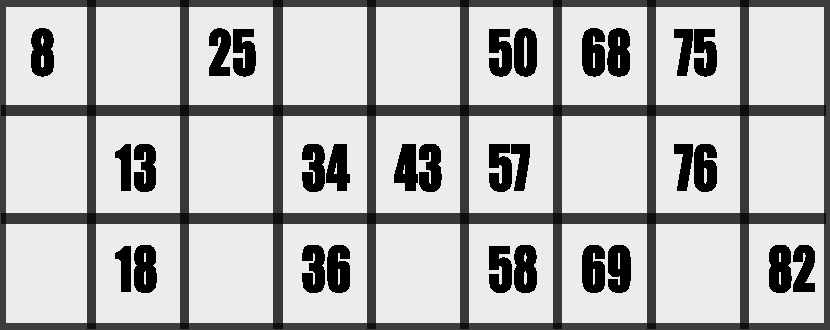
\includegraphics[width=.99\textwidth]{bankoplade.pdf}
\end{center}

Der er vigtige regler for bankoplader.  Her er de\footnote{Nils Andersen.  Hvor
mange bankoplader er der?  2003.\\
\tiny{\url{http://sprutskalle.dk/blog/wp-content/uploads/bankoplader.pdf}}}:

\begin{itemize}
\item Der benyttes numrene fra og med 1 til og med 90.
\item En bankoplade har 3 rækker og 9 søjler.
\item En plade har 15 forskellige numre og 12 tomme felter.
\item Der er mindst et nummer i hver søjle og præcis fem numre i hver række.
\item Den første søjle (fra venstre), kaldt $s_0$, kan have numrene fra og med
$1$ til og med $9$.  Den sidste søjle, kaldt $s_8$, kan have numrene fra og med
$80$ til og med $90$.  Hver søjle $s_n$, hvor $1 \leq n \leq 7$, kan have
numrene fra og med $10n$ til og med $10n + 9$.
\end{itemize}

\textbf{Underopgave 0:} Tjek at den givne eksempelplade opfylder de fem krav.

\textbf{Underopgave 1:} Opfind en algoritme til at komprimere en bankoplade
effektivt, dvs. at repræsentere en bankoplade på få bits (uden tab af
information!).


\newpage

\subsection{Den skægge opgave}

% The Collatz conjecture

Her er en funktion for et vilkårligt tal $n$:
\begin{align*}
f(n) = \begin{cases}
n/2 &\text{hvis }n\text{ er lige}\\
3n + 1 &\text{hvis }n\text{ er ulige}\\
\end{cases}
\end{align*}
For eksempel er $f(10) = 5$ og $f(7) = 22$.

Her er en talfølge -- baseret på funktionen $f$ -- der begynder med et
vilkårligt tal $n$:
\begin{align*}
a_i = \begin{cases}
n &\text{når }i = 0\\
f(a_{i - 1}) &\text{når }i > 0\\
\end{cases}
\end{align*}
Hvis vi for eksempel sætter $n = 12$, får vi talfølgen
$a_0 = 12, a_1 = 6, a_2 = 3, a_3 = 10, a_4 = 5, a_5 = 16, a_6 = 8, a_7 = 4, a_8
= 2, a_9 = 1$.  Vi stopper med at vise en talfølge når den når tallet $1$, for
$1$ er et pænt tal, og $f(f(f(1))) = 1$ (vis dette), så den vil alligevel blot
gentage sig.

\textbf{Din opgave:} Bevis eller modbevis følgende formodning:
\begin{quote}
Ligemeget hvilket starttal $n$ der vælges, vil talfølgen altid nå tallet $1$.
\end{quote}

\textbf{\emph{NB: Der udloddes en flaske snaps til den første som kommer op i
baren med en korrekt besvarelse af denne opgave!}}

\newpage
\begin{flushleft}
\begin{huge}
Barpriser
\end{huge}
\\[.1cm]
\begin{table}[h!]
\begin{tabular}{lr}
\textbf{Øl} & \\
Guld Tuborg / Tuborg Classic (40 cl på fad) & 15 kr.\\
BMC India Pale Ale (40 cl på fad) & 20 kr.\\[2ex]
\textbf{Drinks} & \\
Gin \& Tonic (eller Lemon) & 20 kr.\\
Rom \& Cola & 20 kr.\\
White Russian & 25 kr.\\
Shot (2 cl) & 10 kr.\\[2ex]
\textbf{Diverse} & \\
Klippekort af værdi 120 kr. & 100 kr.\\
Vin (flaske) & 45 kr.\\
Snaps (35 cl) & 50 kr.\\
Somersby (33 cl på dåse) & 15 kr. \\
Sodavand (50 cl på flaske) & 10 kr.\\
\end{tabular}
\end{table}
\end{flushleft}
\vfill
\begin{center}

\includegraphics[width=.9\linewidth]{supwiz.pdf}
\\[2mm]\emph{SupWiz sponserer billigere ølpriser i baren i år.}
\end{center}


\end{document}

